\documentclass{beamer}
\usetheme{Hannover} 
\usepackage{graphicx}
\graphicspath{ {./Zdjęcia/} }
\usepackage[polish]{babel}
\usepackage[utf8]{inputenc}
\usepackage[T1]{fontenc}           


\DeclareGraphicsExtensions{.png,.jpg,.pdf,.mps}
\setbeamertemplate{footline}[frame number]
\title{Różnice pomiędzy różnymi rodzajami silników}
\author{Bartosz Kałmuczak, Stanisław Koprowski, Andrzej Kowalski} 
\institute{Politechnika Poznańska}

\AtBeginSection[]
{
	\begin{frame} 
	\frametitle{Spis treci} 
	\tableofcontents[currentsection]  
	\end{frame}
} 

\begin{document}
	\begin{frame} 
		\titlepage
	\end{frame}

\section{Podstawa - silnik spalinowy}

	\begin{frame} 
	\frametitle{Podział na rodzaj zapłonu}

		\begin{columns}

			\begin{column}{0.5\textwidth}
			\pause Silniki z zapłonem iskrowym

				\begin{itemize}
				\pause \item Stosunkowo lekka konstrukcja
				\pause \item Szybkobieżne
				\pause \item Prosta konstrukcja
				\end{itemize}

			\end{column}

			\begin{column}{0.5\textwidth}
			\pause Silniki z zapłonem samoczynnym

				\begin{itemize}
				\pause \item Mniejsze spalanie
				\pause \item Duża niezawodność
				\pause \item Bezpieczniejsze paliwo
				\end{itemize}
			\end{column}
		\end{columns}



	\end{frame}
	\begin{frame}

	\frametitle{Podział na cykl pracy}
		\begin{columns} 
			\begin{column}{0.5\textwidth}
				\pause \Large Cykl dwusuwowy
				\begin{itemize}
					\small \pause \item 1. Suw Sprężania
					\item \small 2. Suw Pracy
				\end{itemize}
			\end{column}

			\begin{column}{0.5\textwidth}
			\pause \Large Cykl czterosuwowy
				\begin{itemize}
				\small \pause \item 1. Suw ssania
				\item \small 2. Suw Sprężania
				\item \small 3. Suw Pracy
				\item \small 4.Suw wydechu
				\end{itemize}
			\end{column}
		\end{columns}
 	\end{frame}
	\begin{frame}
	
	\frametitle{Przykładowe budowy}
		\begin{columns}
			\begin{column}{0.5\textwidth}
				\pause 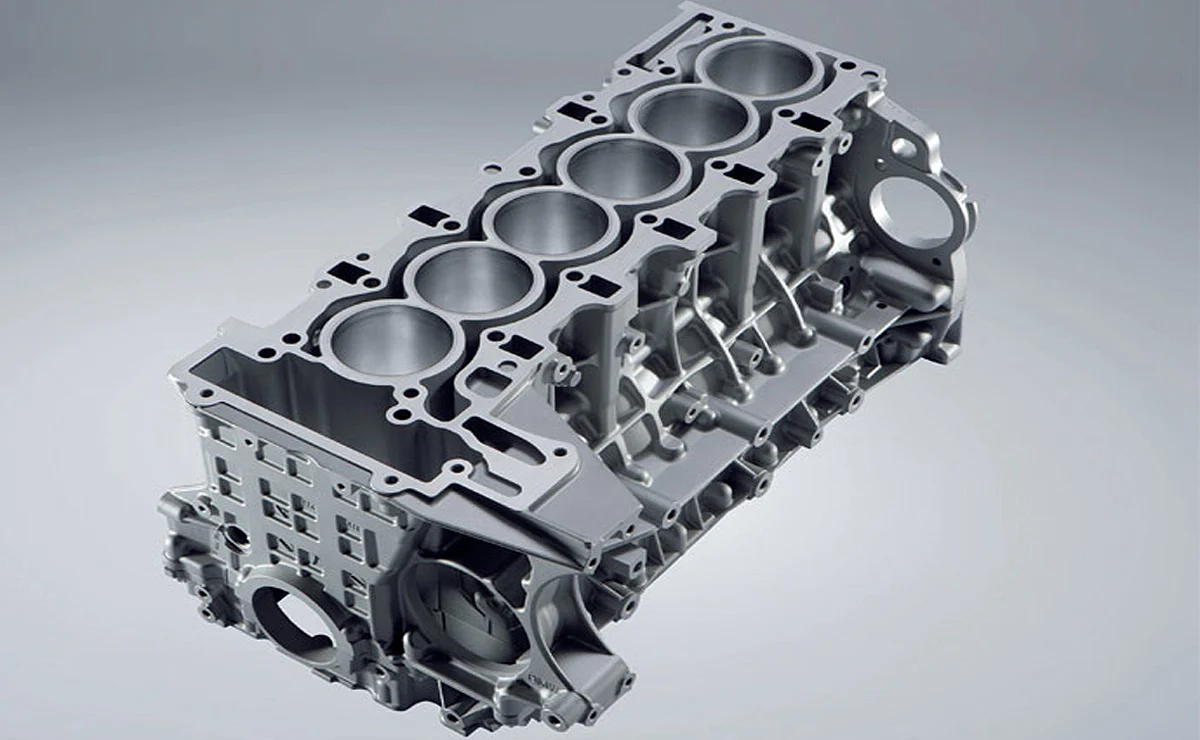
\includegraphics[width=2.5cm,height=2.5cm]{Inline}
				\pause 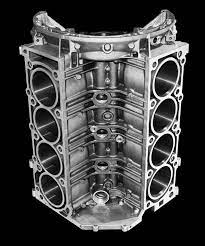
\includegraphics[width=2.5cm,height=2.5cm]{V}
				\pause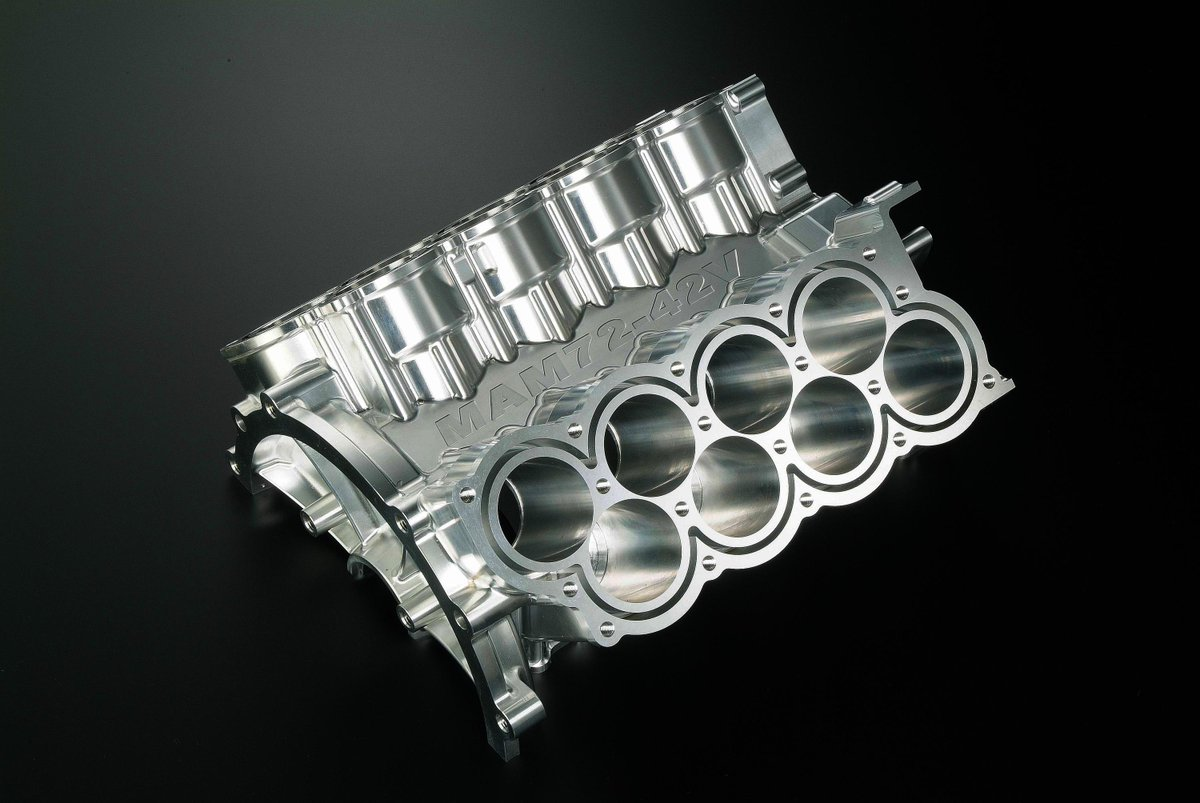
\includegraphics[width=2.5cm,height=2.5cm]{W}
			\end{column}
			
			\begin{column}{0.5\textwidth}
				\pause\includegraphics[width=2.5cm,height=2.5cm]{radial}
				\pause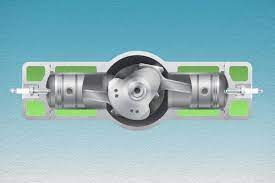
\includegraphics[width=2.5cm,height=2.5cm]{boxer}
				\pause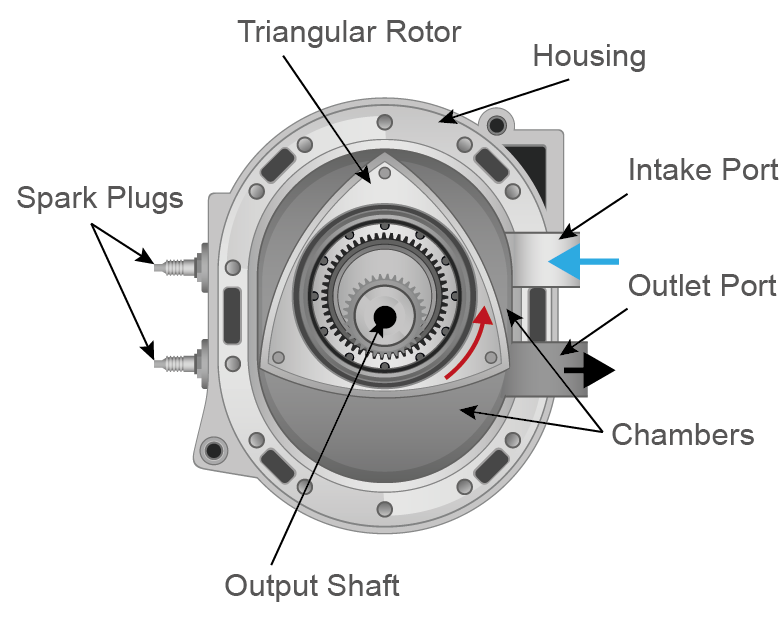
\includegraphics[width=2.5cm,height=2.5cm]{Wankel}
			\end{column}
		\end{columns}
	\end{frame}
	
\section{Ważny punkt w prezentacji} 

\begin{frame}
\frametitle{Nagłówek 3}
Treśc slajdu

\pause Piszemy dalej, opowiadamy, wyjaśniamy.

\pause \begin{block} {Ważna definicja}
Funkcja  $y$ jest bardzo istotna, więc nie można jej pominąć.
\end{block}
\end{frame}

\begin{frame}
\frametitle{Klika przykłóadów bloków}
\begin{block}{Tytuł bloku}
Blok zwykły - kolor zależy od schematu kolorów
\end{block}
\begin{alertblock}{To jest Alertblock}
Styl jest zależny od ustawień koloru obiektu \alert{alert}
\end{alertblock}
\begin{examples}
Zawsze zielony, nie ma możliwości zmiany koloru
\end{examples}
\end{frame}

\begin{frame}
\frametitle{Kolejny slajd}
Totaj opisujemy kolejny slajd

Możemy dodawać różne elementy, np. wzory

$$ g(x)=
\begin{cases}
0.5x+x^2\sin(1/x), &\text{if }x\neq0 \\
0, &\text{if }x=0
\end{cases}
$$
\end{frame}

\section{Podsumowanie}

\begin{frame}
Tu możemy napisać wnioski.

\vspace{.5cm}

Jeszcze jeden wniosek
\vspace{.5cm}

I jeszcze jeden (ostatni).
\vspace{2cm}


\pause
\textbf{\textcolor{blue}{Dziękuję za uwagę.}}
\end{frame}



\end{document}

